\documentclass[11pt, a4paper]{article}
\usepackage{pdfpages}
\usepackage{parallel}
\usepackage[T2A]{fontenc}
\usepackage{ucs}
\usepackage[utf8x]{inputenc}
\usepackage[polish,english,russian]{babel}
\usepackage{hyperref}
\usepackage{rotating}
\usepackage[inner=2cm,top=1.8cm,outer=2cm,bottom=2.3cm,nohead]{geometry}
\usepackage{listings}
\usepackage{graphicx}
\usepackage{wrapfig}
\usepackage{longtable}
\usepackage{indentfirst}
\usepackage{array}
\usepackage{tikzsymbols}
\usepackage{soul}
\usepackage[ruled,vlined]{algorithm2e}
%\counterwithout{figure}{section} 

\usepackage{url}
\makeatletter
\g@addto@macro{\UrlBreaks}{\UrlOrds}
\makeatother

\newcolumntype{P}[1]{>{\raggedright\arraybackslash}p{#1}}
\frenchspacing
\usepackage{fixltx2e} %text sub- and superscripts
\usepackage{icomma} % коскі ў матэматычным рэжыме
\PreloadUnicodePage{4}

\newcommand{\longpage}{\enlargethispage{\baselineskip}}
\newcommand{\shortpage}{\enlargethispage{-\baselineskip}}

\def\switchlang#1{\expandafter\csname switchlang#1\endcsname}
\def\switchlangbe{
\let\saverefname=\refname%
\def\refname{Літаратура}%
\def\figurename{Іл.}%
}
\def\switchlangen{
\let\saverefname=\refname%
\def\refname{References}%
\def\figurename{Fig.}%
}
\def\switchlangru{
\let\saverefname=\refname%
\let\savefigurename=\figurename%
\def\refname{Литература}%
\def\figurename{Рис.}%
}

\hyphenation{admi-ni-stra-tive}
\hyphenation{ex-pe-ri-ence}
\hyphenation{fle-xi-bi-li-ty}
\hyphenation{Py-thon}
\hyphenation{ma-the-ma-ti-cal}
\hyphenation{re-ported}
\hyphenation{imp-le-menta-tions}
\hyphenation{pro-vides}
\hyphenation{en-gi-neering}
\hyphenation{com-pa-ti-bi-li-ty}
\hyphenation{im-pos-sible}
\hyphenation{desk-top}
\hyphenation{elec-tro-nic}
\hyphenation{com-pa-ny}
\hyphenation{de-ve-lop-ment}
\hyphenation{de-ve-loping}
\hyphenation{de-ve-lop}
\hyphenation{da-ta-ba-se}
\hyphenation{plat-forms}
\hyphenation{or-ga-ni-za-tion}
\hyphenation{pro-gramming}
\hyphenation{in-stru-ments}
\hyphenation{Li-nux}
\hyphenation{sour-ce}
\hyphenation{en-vi-ron-ment}
\hyphenation{Te-le-pathy}
\hyphenation{Li-nux-ov-ka}
\hyphenation{Open-BSD}
\hyphenation{Free-BSD}
\hyphenation{men-ti-on-ed}
\hyphenation{app-li-ca-tion}

\def\progref!#1!{\texttt{#1}}
\renewcommand{\arraystretch}{2} %Іначай формулы ў матрыцы зліпаюцца з лініямі
\usepackage{array}

\def\interview #1 (#2), #3, #4, #5\par{

\section[#1, #3, #4]{#1 -- #3, #4}
\def\qname{LVEE}
\def\aname{#1}
\def\q ##1\par{{\noindent \bf \qname: ##1 }\par}
\def\a{{\noindent \bf \aname: } \def\qname{L}\def\aname{#2}}
}

\def\interview* #1 (#2), #3, #4, #5\par{

\section*{#1\\{\small\rm #3, #4. #5}}
\ifx\ParallelWhichBox\undefined%
    \addcontentsline{toc}{section}{#1, #3, #4}%
\else%
\ifnum\ParallelWhichBox=0%
    \addcontentsline{toc}{section}{#1, #3, #4}%
\fi\fi%

\def\qname{LVEE}
\def\aname{#1}
\def\q ##1\par{{\noindent \bf \qname: ##1 }\par}
\def\a{{\noindent \bf \aname: } \def\qname{L}\def\aname{#2}}
}

\newcommand{\interviewfooter}[1]{
\vskip 1em
\noindent \textit{#1}
}

\switchlang{en}
\begin{document}

\title{1989 "--- Fujitsu FM Towns model 1 mouse (FMT-MO101)}
\date{}
\author{~}
\maketitle
\selectlanguage{english}

In February 1989, Fujitsu announced the first model of the FM Towns family of computers, running its own Towns OS graphics system. FM Towns was a proprietary variant of the PC-compatible architecture focused on multimedia applications and games. The first FM Towns model used an Intel 80386 processor, was equipped with 1 or 2 megabytes of RAM, a CD-ROM drive, a microphone, a gamepad and a mouse. The mouse that came with this model is the Fujitsu FMT-MO101 (fig. \ref{fig:FMT1Pic}).

\begin{figure}[h]
   \centering
    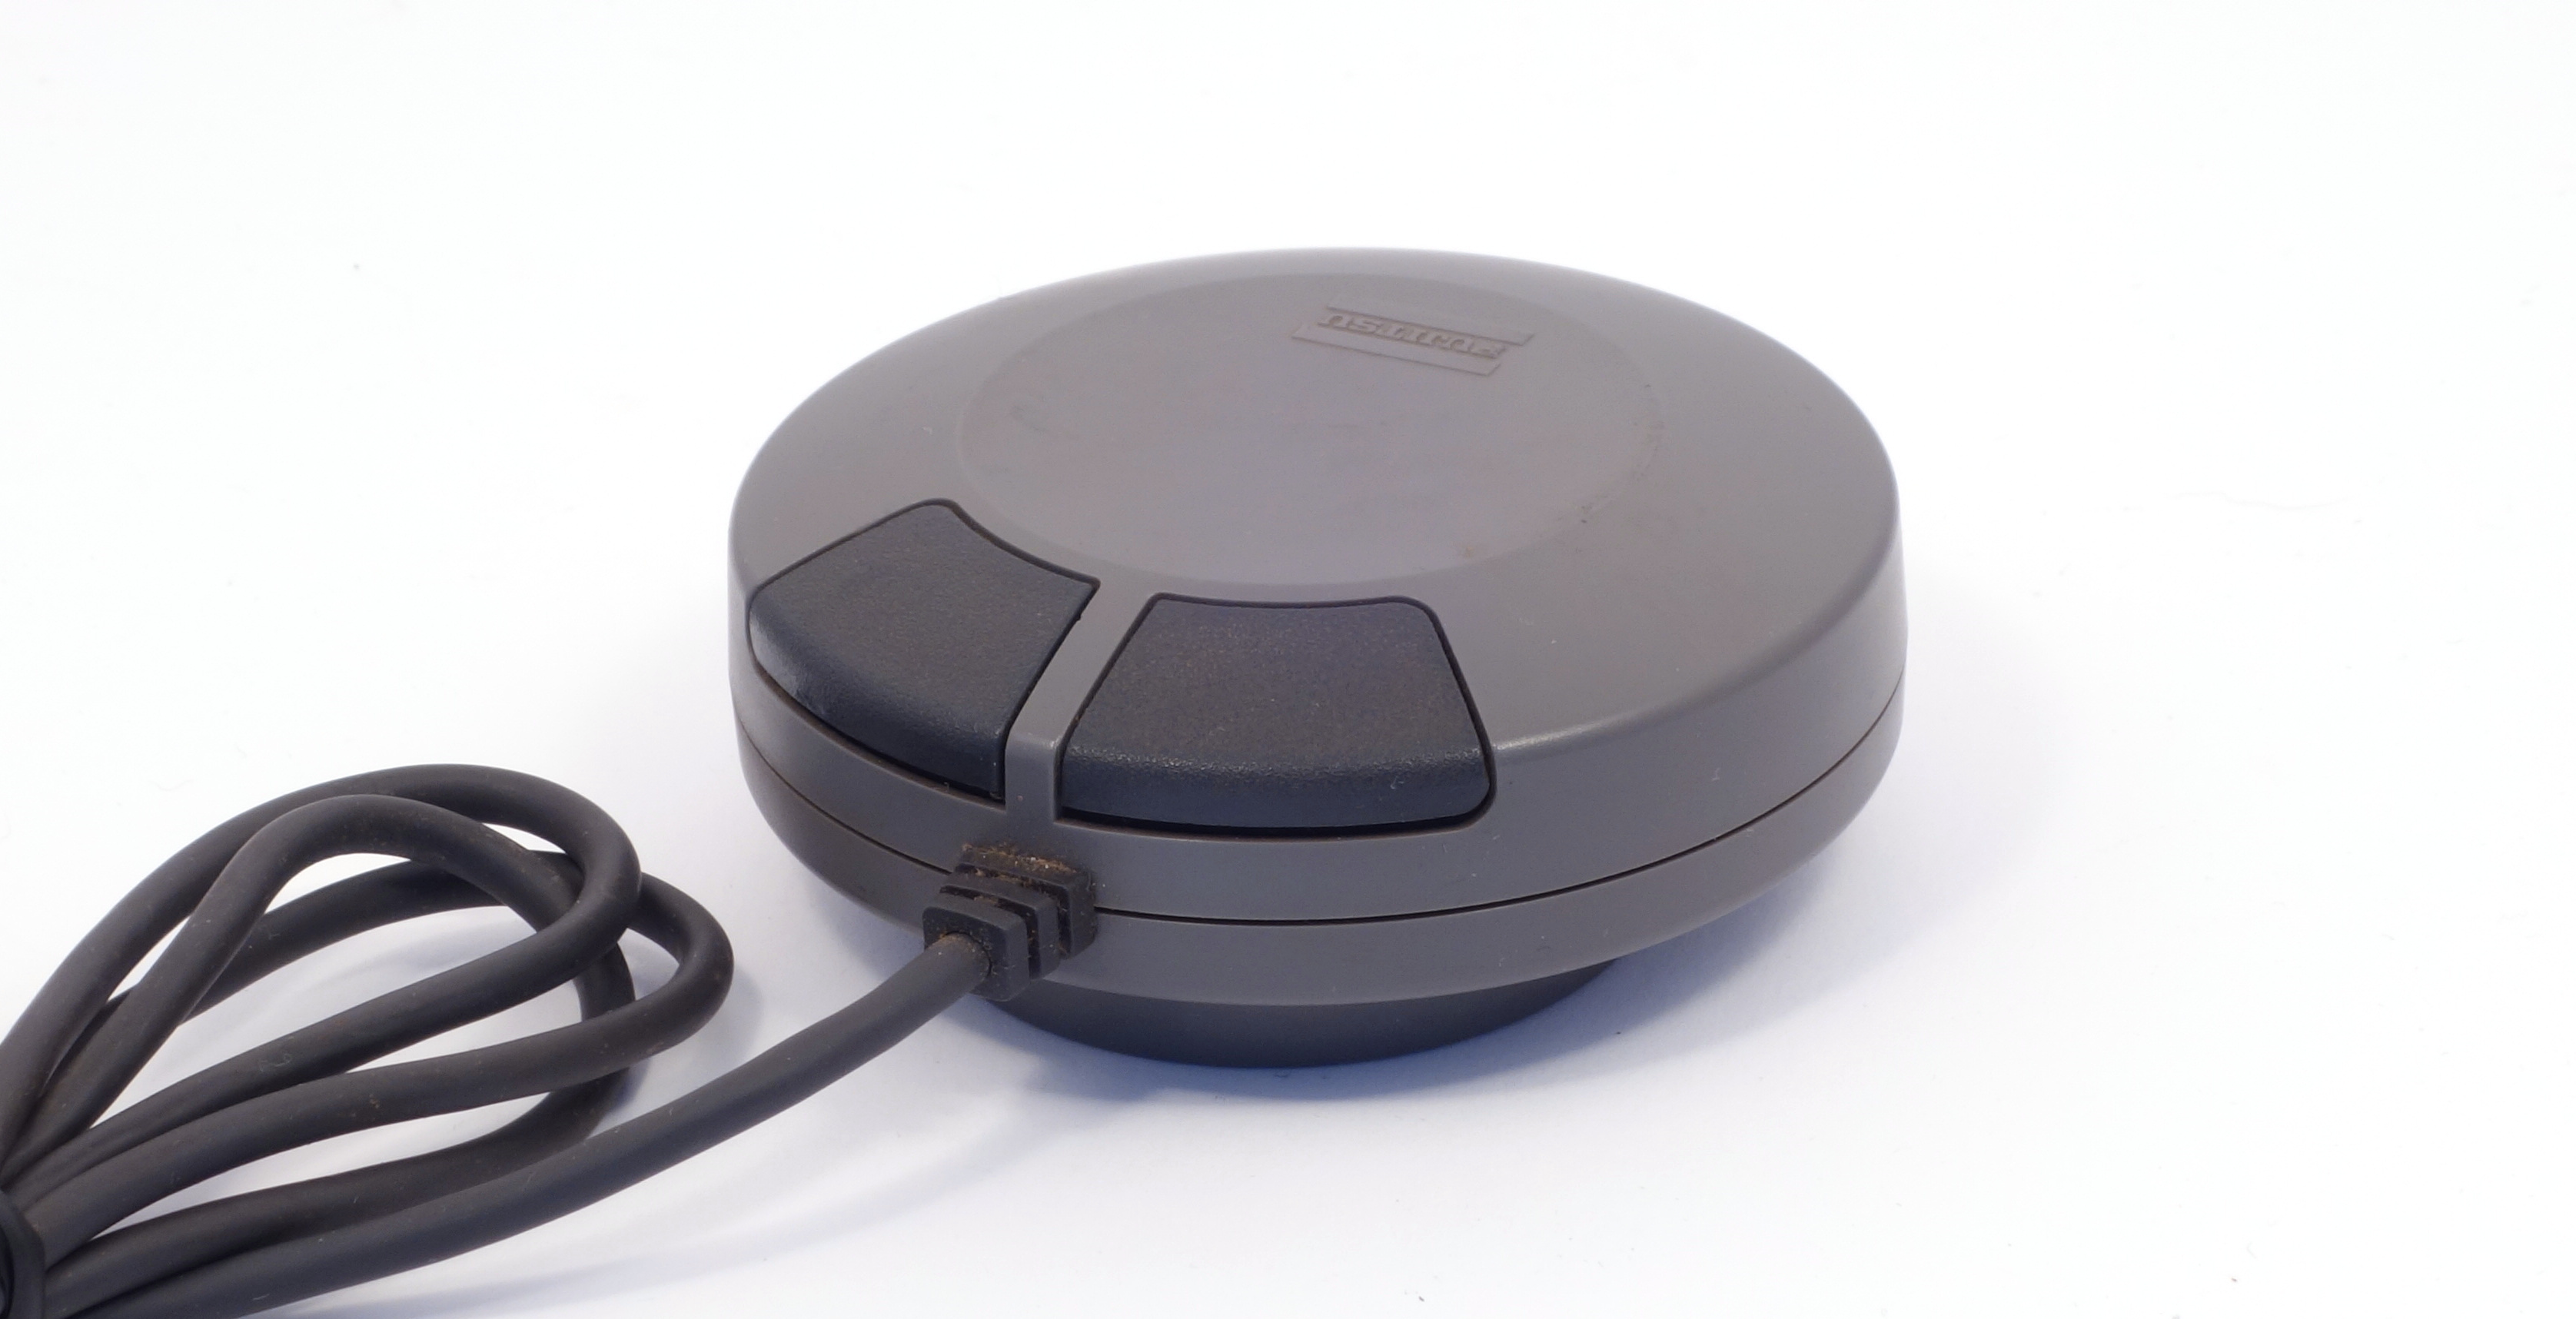
\includegraphics[scale=0.6]{1989_fujitsu_fmt_mo101_mouse/pic_30.jpg}
    \caption{Fujitsu FMT-MO101 mouse}
    \label{fig:FMT1Pic}
\end{figure}

Of course, the main feature of this mouse is its round shape (or it would be more accurate to call its body mushroom-shaped). Two fairly large buttons made of darker plastic in the form of sectors are located in the front of the case. You can also see the embossed Fujitsu logo on the top side of the case \cite{twinklemagic}. The bottom of the mouse has a more traditional look, including low-friction feet and a removable latch ring that allows the user to remove the ball for cleaning. In general, the case design can definitely be described as memorable and aesthetically pleasing.

\begin{figure}[h]
    \centering
    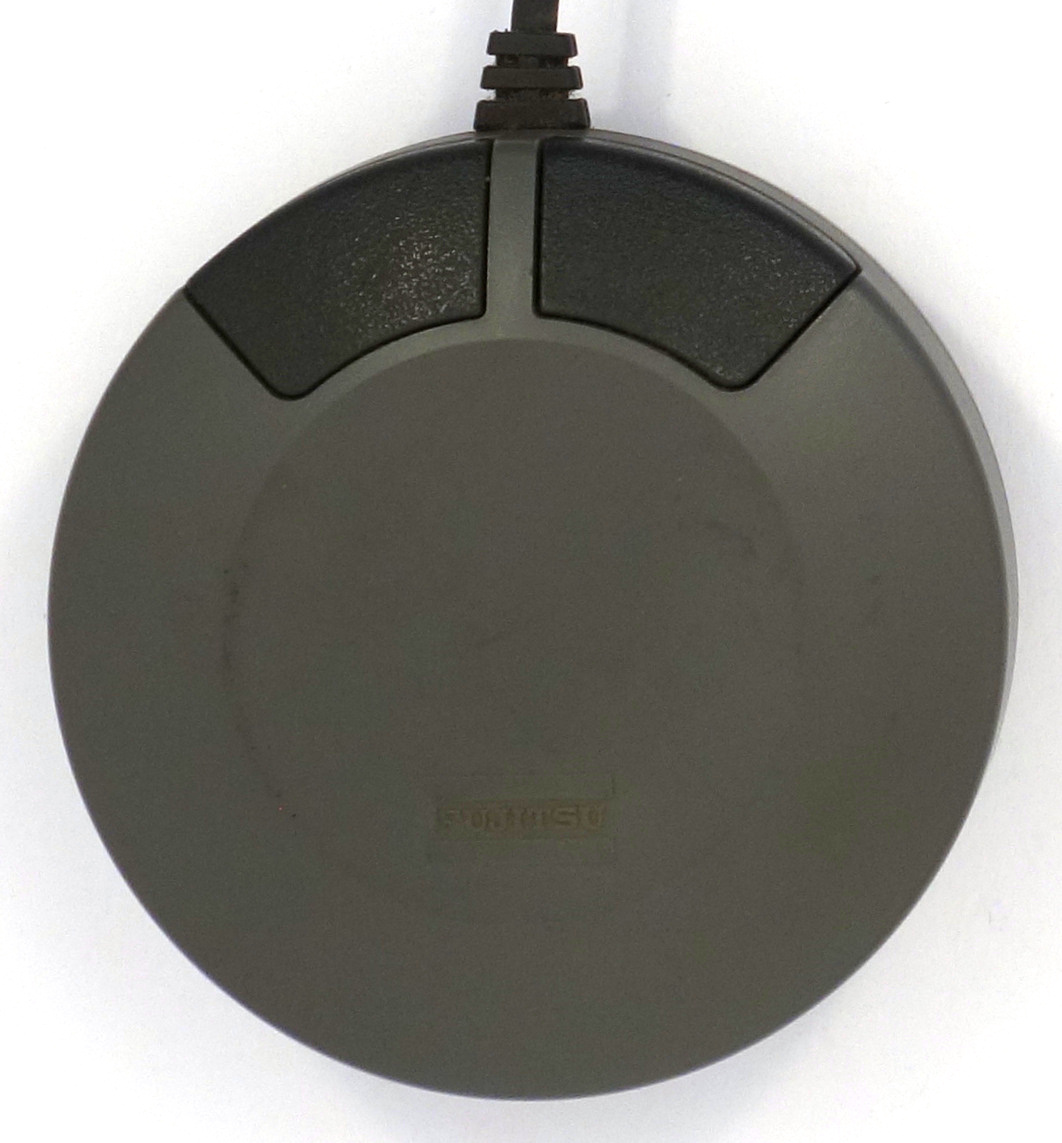
\includegraphics[scale=0.55]{1989_fujitsu_fmt_mo101_mouse/top_30.jpg}
    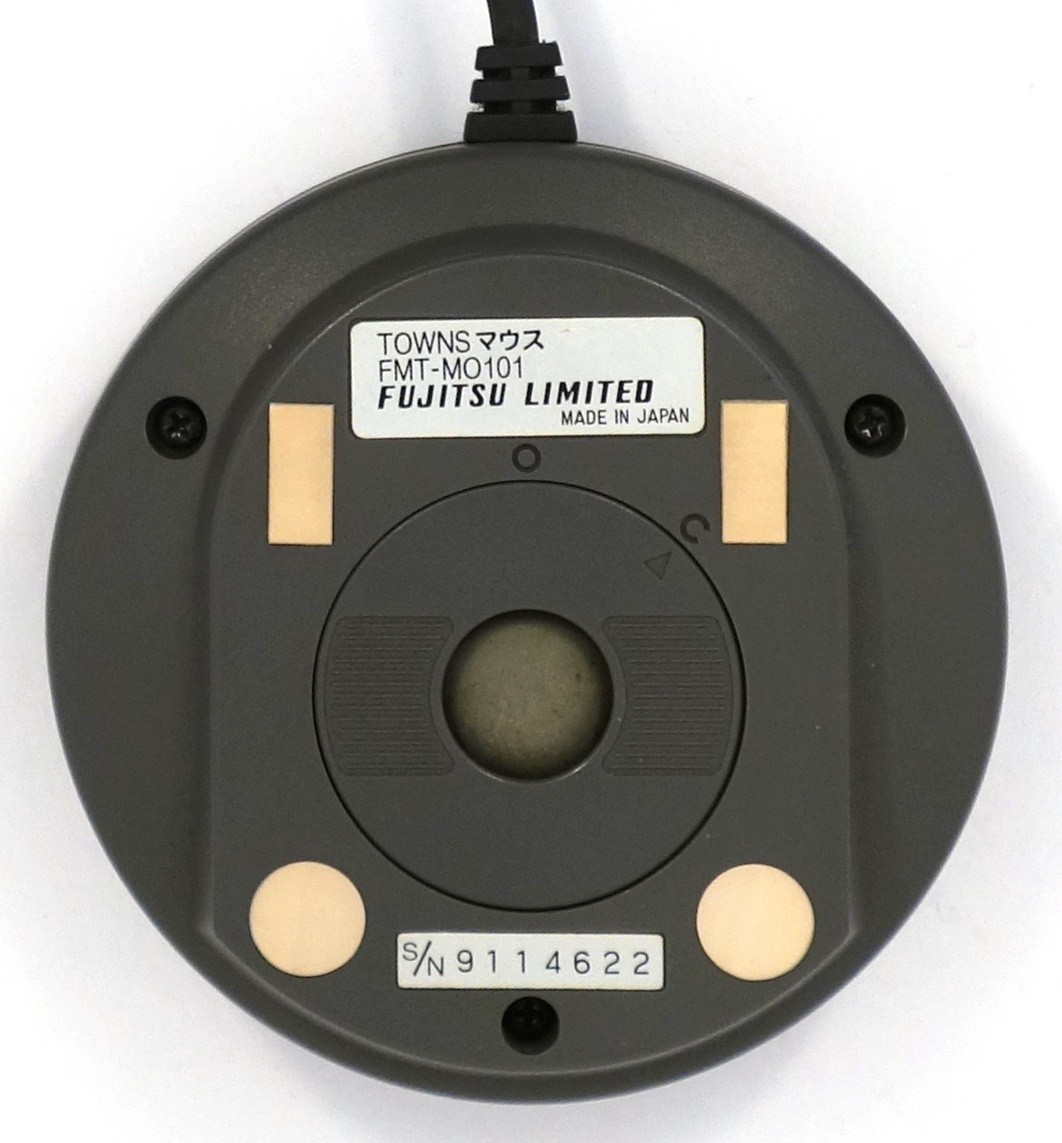
\includegraphics[scale=0.55]{1989_fujitsu_fmt_mo101_mouse/bottom_30.jpg}
    \caption{Fujitsu FMT-MO101 mouse, top and bottom views}
    \label{fig:FMT1TopAndBottom}
\end{figure}

The mouse is medium in size, which, combined with the round shape, makes it too wide \cite{twinklemagic} for a comfortable grip (fig. \ref{fig:FMT1Size}, \ref{fig:FMT1Hand}).

\begin{figure}[h]
    \centering
    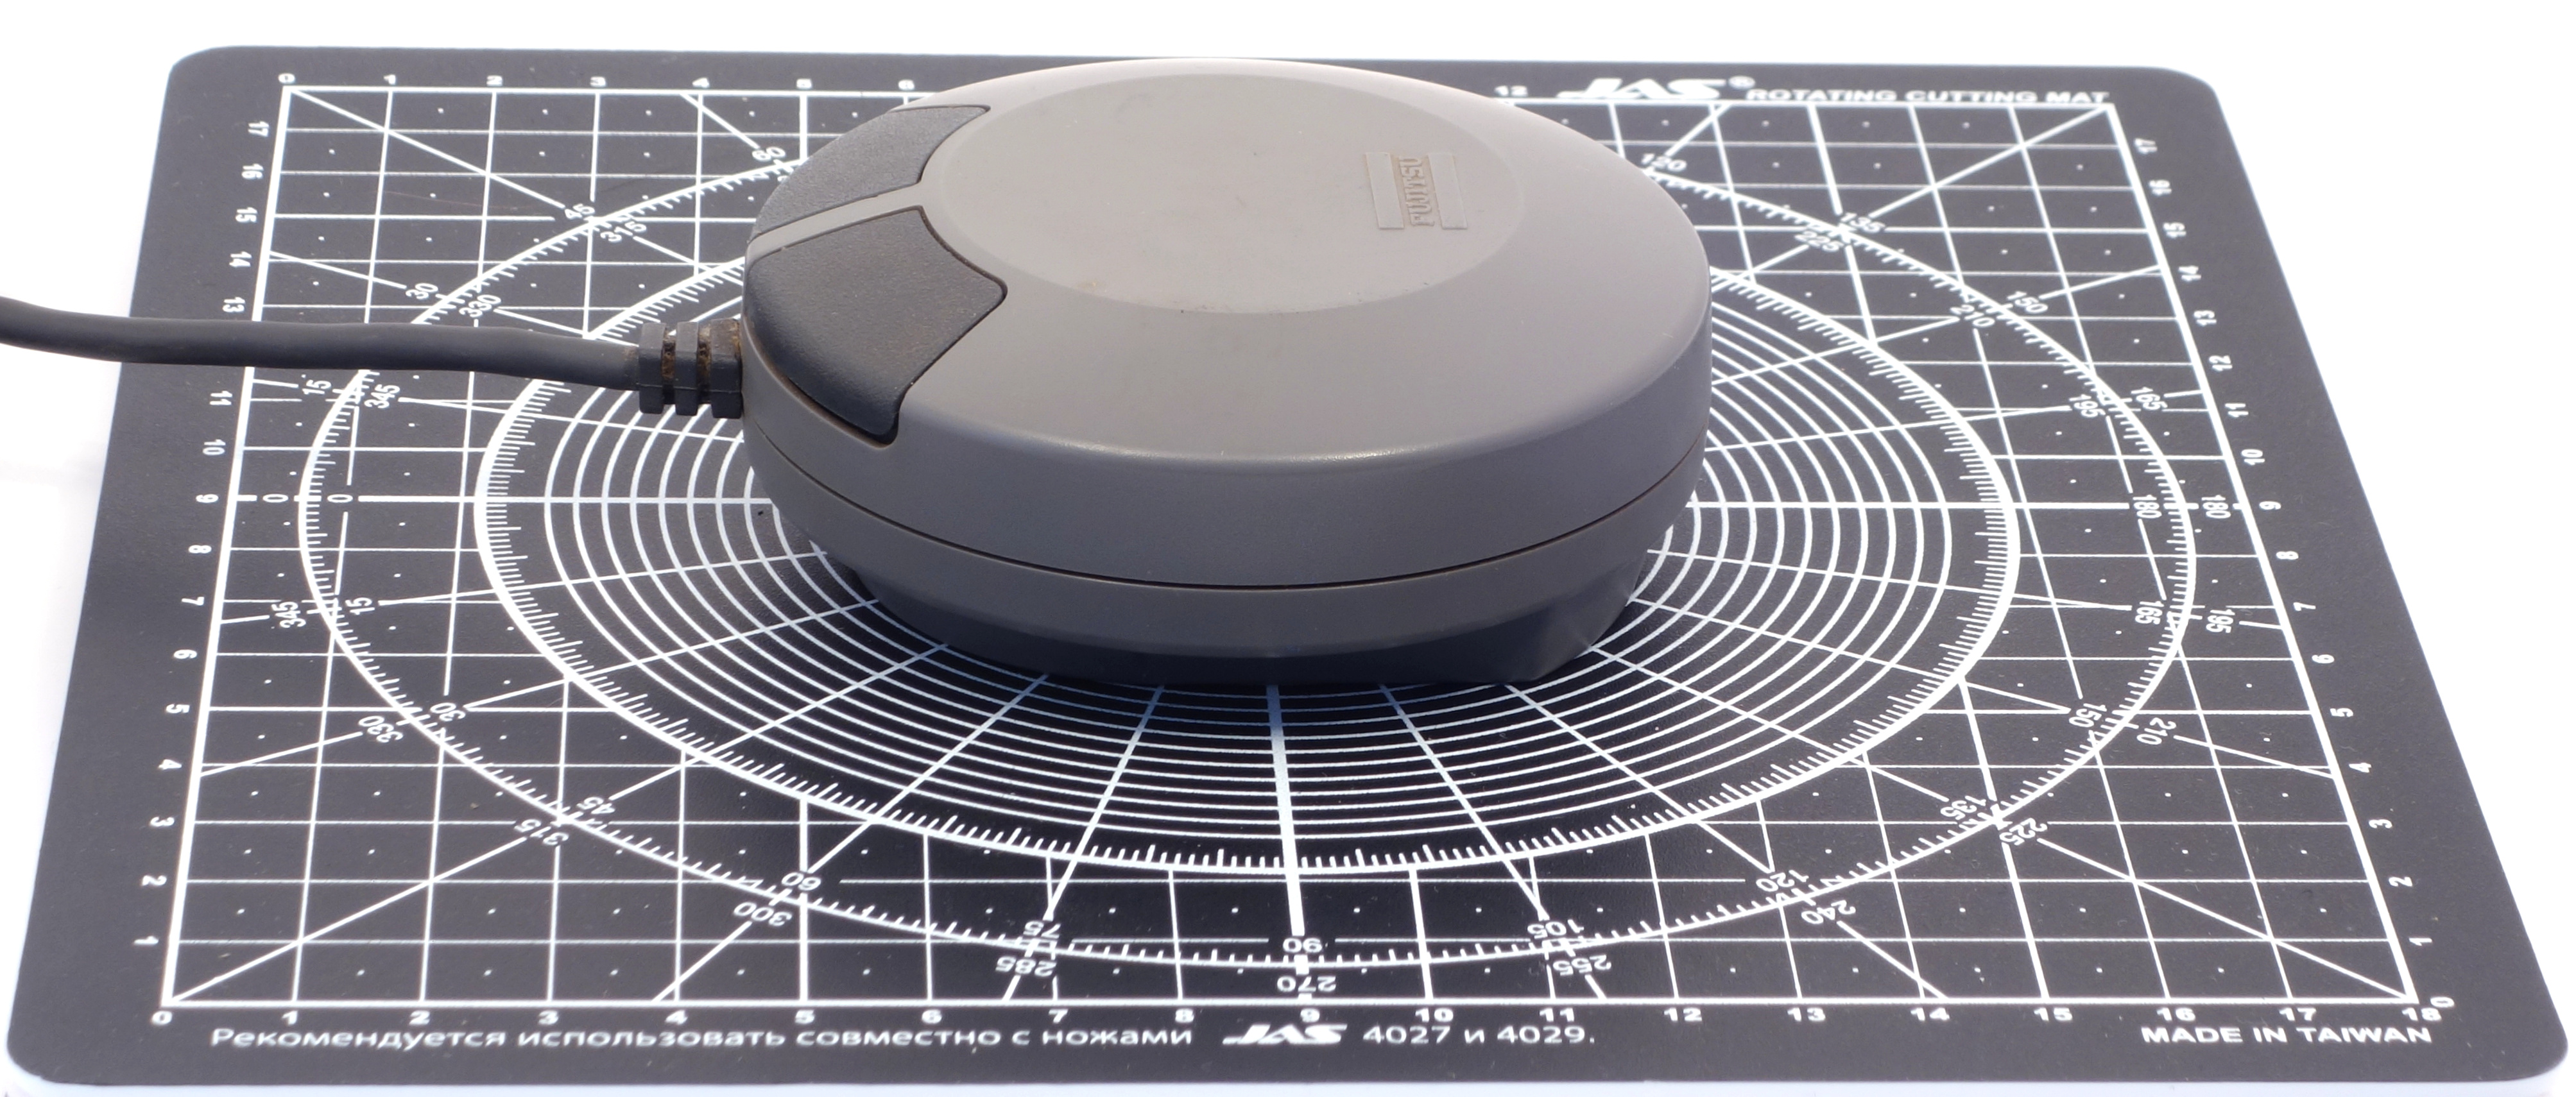
\includegraphics[scale=0.48]{1989_fujitsu_fmt_mo101_mouse/size_30.jpg}
    \caption{Fujitsu FMT-MO101 mouse on a graduated pad with a grid step of 1~cm}
    \label{fig:FMT1Size}
\end{figure}

It is also obvious that the narrower chassis base does not add stability to the mouse. This problem is not significant, but nevertheless, the user instinctively tries to lean less on the side edges, for fear of inadvertently knocking over the mouse. Probably for this reasons, subsequent FM Towns computer mice had less noticeable but more practical shape.

\begin{figure}[h]
    \centering
    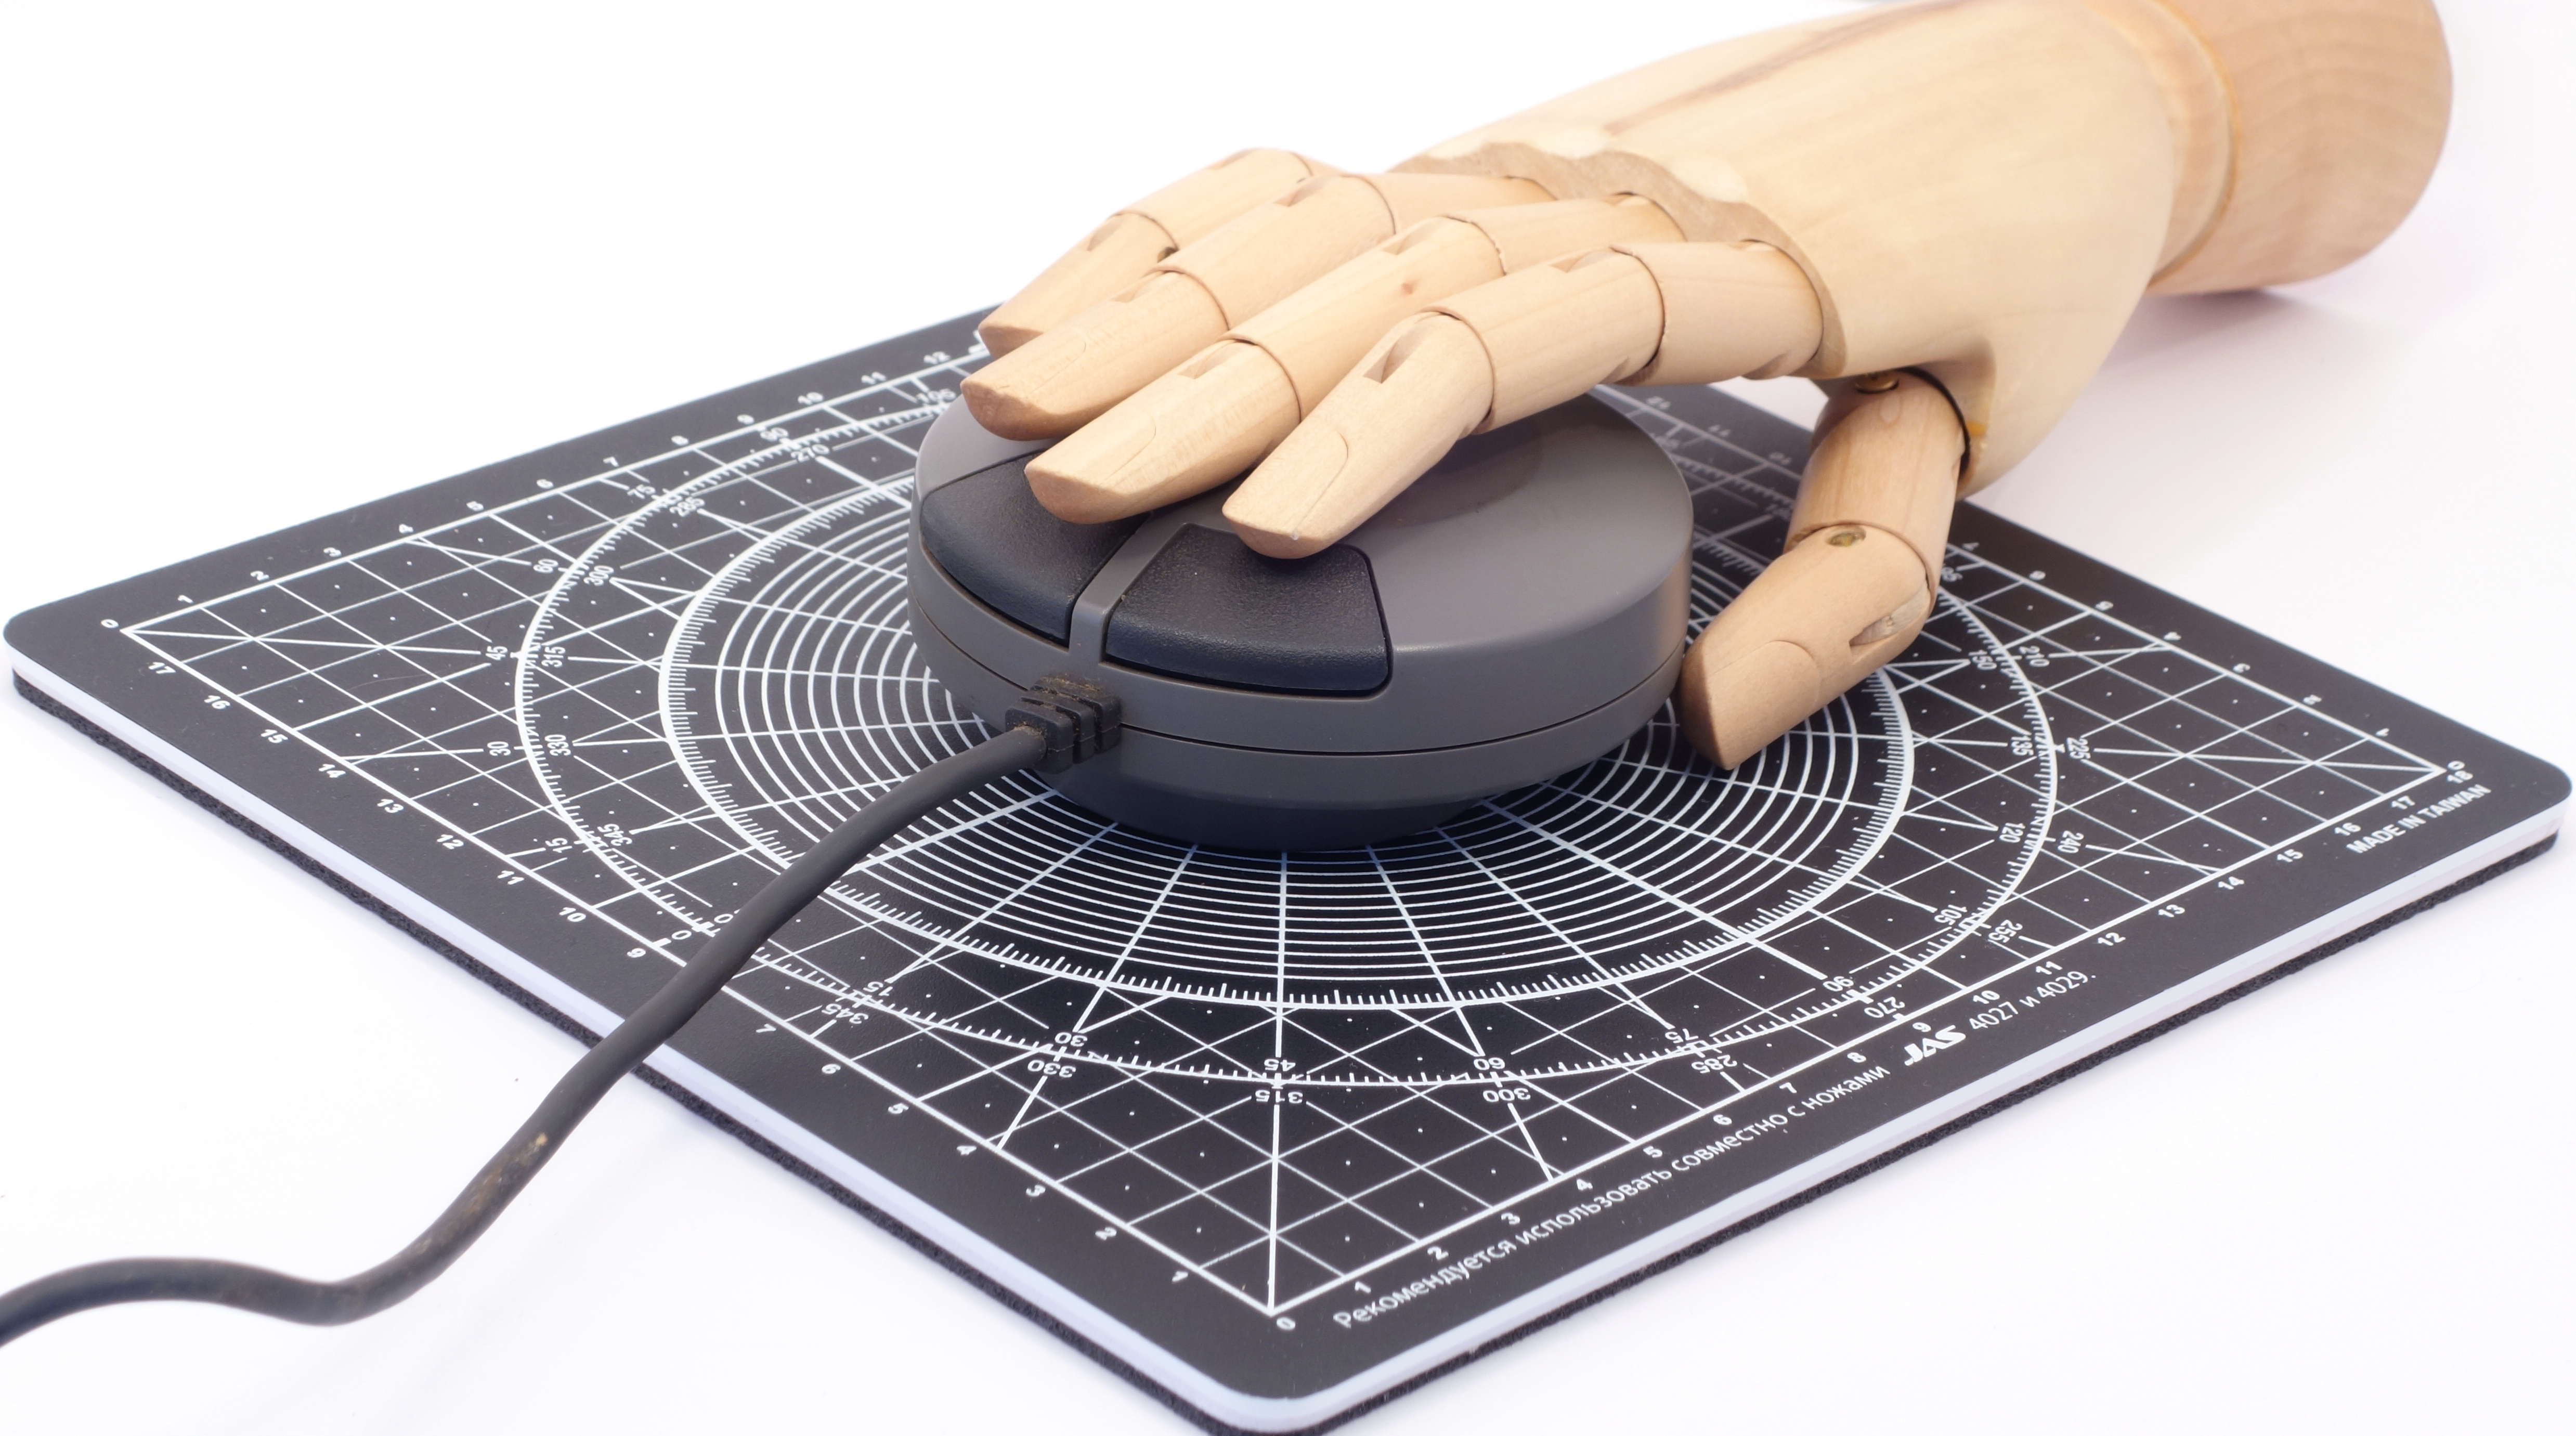
\includegraphics[scale=0.47]{1989_fujitsu_fmt_mo101_mouse/hand_30.jpg}
    \caption{Fujitsu FMT-MO101 mouse with a human hand model}
    \label{fig:FMT1Hand}
\end{figure}

From a technical point of view, the FM Towns mouse has an MSX interface, which makes it quite universal in terms of \cite{tepatti} compatibility.

The internals of the mouse shown in fig. \ref{fig:FMT1inside} make it possible to classify it as optomechanical. The implementation is quite advanced for its time. At the same time, metal encoder disks attract attention, because they are more typical for expensive mice of the early 80s (for example, Depraz mice).

\begin{figure}[h]
    \centering
    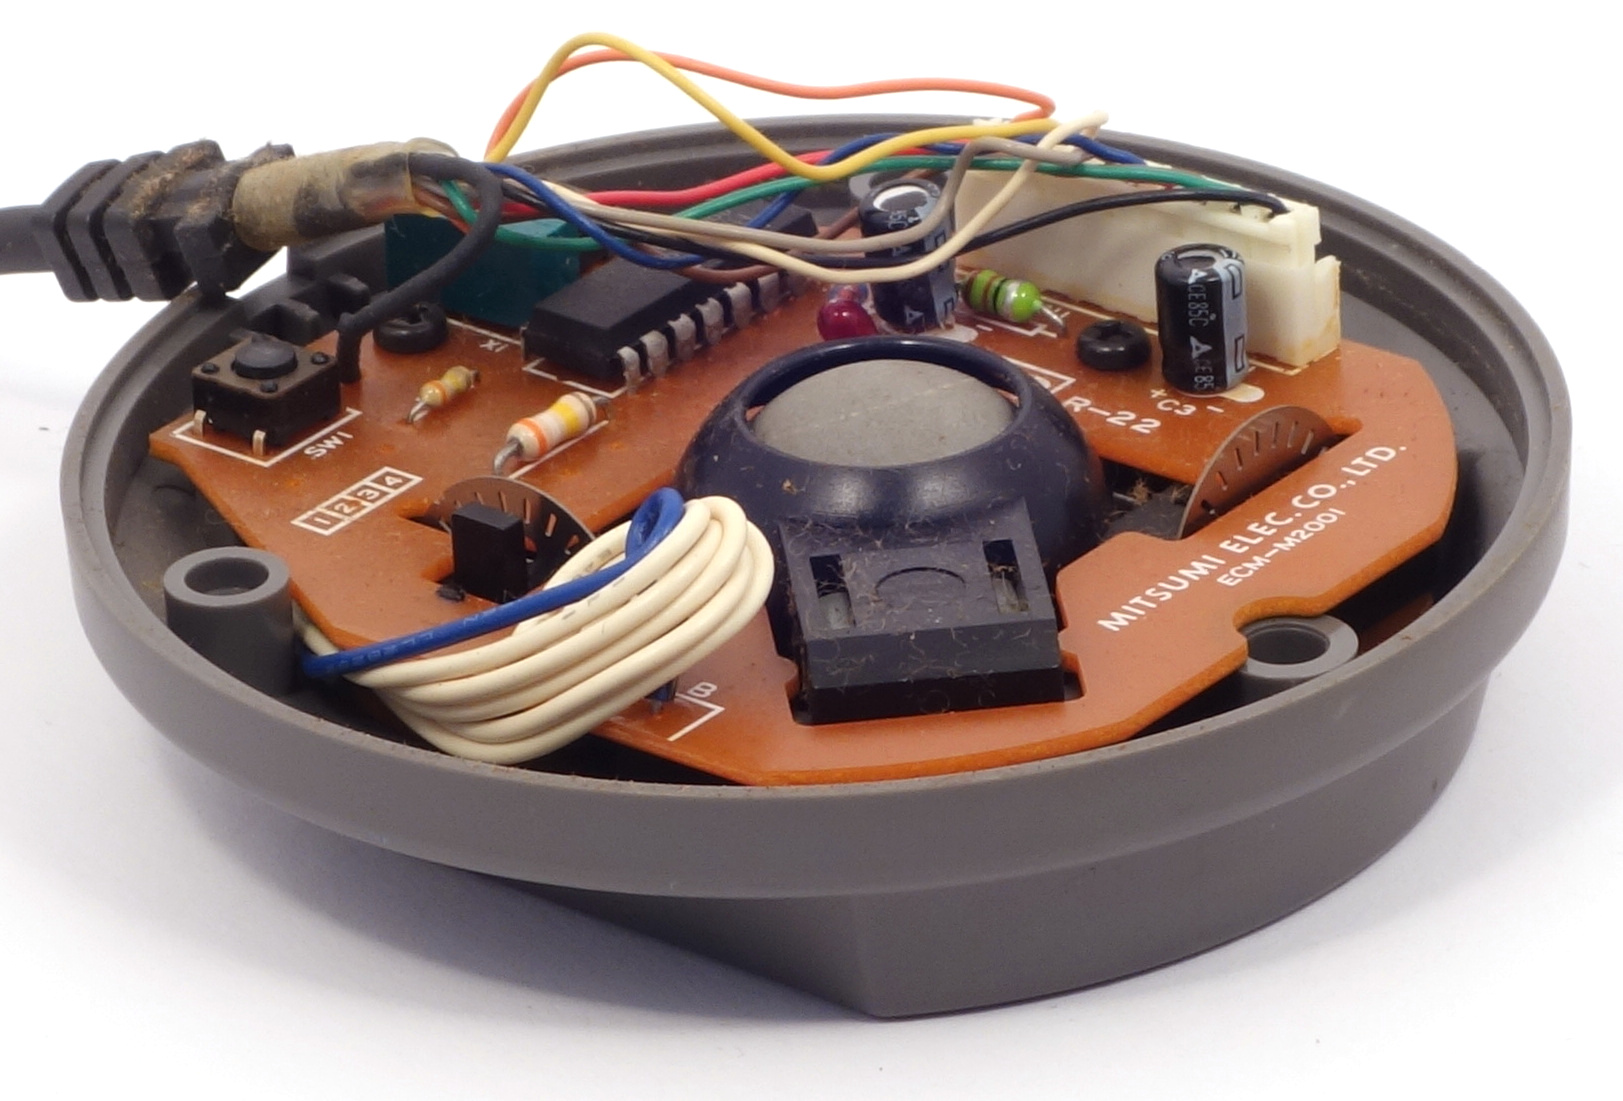
\includegraphics[scale=0.8]{1989_fujitsu_fmt_mo101_mouse/inside_30.jpg}
    \caption{Fujitsu FMT-MO101 mouse disassembled}
    \label{fig:FMT1Inside}
\end{figure}


\begin{thebibliography}{9}
    \bibitem{wikipedia} FM Towns \url{https://en.wikipedia.org/wiki/FM_Towns}
    \bibitem{twinklemagic} Mouse to mouse \url{http://twinklemagic.la.coocan.jp/towns/mouse/MOUSE_to_MOUSE.html} 
    \bibitem{tepatti} Tepatti T. FM Towns Keyboards, Mice, and Game Pads \url{https://tepatti.com/blog/005/index.html}
\end{thebibliography}
\end{document}
